\chapter{Introduction}

Water is a fundamental molecule that plays an important role in numerous biological, chemical, environmental, and industrial processes~\cite{henry2005state,Kurz2008,ahuja2013green}.
Water is ubiquitous, comprising two-thirds of the Earth's surface and about half the volume of every living biological cell~\cite{Kontogeorgis2022,ling2004determines}. Its unusual properties include a strong network of hydrogen bonds, which directly correlates to a high boiling point, strong cohesion, high surface tension, high heat of vaporization, and low vapor pressure. Additionally, ice has a lower density than liquid water, and water is an excellent solvent due to its polar nature, which allows it to dissolve a wide range of substances. These characteristics make water an excellent medium for chemical reactions and biological processes~\cite{Kontogeorgis2022,brini2017water}.

Due to its high cohesion, water can easily form surfaces and boundaries. Water interfaces have important applications in heterogeneous catalysis~\cite{fechete2012past}, fuel cells~\cite{Owejan2009}, and protein folding~\cite{levy2006water}. In particular, aqueous solutions containing salts affect electrochemical gradients, which play an important role in cell membrane regulation~\cite{lai2006distribution}. Despite extensive research on both experimental and theoretical fronts, accurately modeling the structural and dynamical properties of salt solutions remains a challenge. For example, the concentration of electrolytic salts affects the surface tension of water, as shown in Figure~\ref{fig:surf_tens_solute}, where different trends are observed for different chemical species. For instance, salts containing divalent cations exhibit a steeper upward slope in surface tension than those with monovalent cations. Moreover, the surface tension starts to plateau at higher concentrations for some salts, such as \ch{NaBr}, \ch{KI}, \ch{NaI}, and \ch{NH_4Cl}.

Significant efforts have been devoted to developing models to reproduce the behavior of water in computer simulations. The most widely employed models for water are empirical models, whose parameters are obtained by fitting to experimentally measured properties~\cite{Duin2001,brenner2002second,daw1984embedded}. While empirical models provide a practical and efficient way to simulate large systems, they are limited by their transferability to different chemical environments, sensitivity to the parameters used, rigidity—since they assume fixed bond lengths, angles, and dihedral angles based on equilibrium positions—and accuracy, due to neglecting polarization and quantum effects.  In contrast, ab initio models are determined from first principles and therefore do not require fitting to experimental data~\cite{car1985unified,Marx2009,kohn1965self}. However, \emph{ab initio} models are computationally expensive because they require solving the electronic structure problem at each molecular dynamics simulation step, which greatly limits the system size to a few hundred atoms and the simulation timescale to a few picoseconds.

Nevertheless, recent advances in machine learning (ML) have enabled the development of deep neural network (DNN) potentials that can predict a plethora of material properties with the same accuracy as the underlying \emph{ab initio} theory but with the efficiency of empirical methods~\cite{Thompson2015,Huan2017,Behler2007,Behler2016,Chmiela2017,Unke2021}. Machine learning methods aim to learn the functional relationship between inputs (chemical descriptors) and outputs (properties) from patterns or structures in the data, which ideally reflect the underlying effective “rules” of quantum mechanics~\cite{schutt2020machine}.

This thesis focuses on the properties of neat water (without any solutes) at an interface and simulates relevant properties such as surface tension, density, and dipole orientation using deep neural network potentials trained on bulk and interface data. Specifically, the objectives are:

\begin{itemize}
      \item To develop accurate and transferrable DeepNN potentials for
            interfaces
      \item To explore the quality of the training data set in improving the
            description of water interfaces
      \item To understand reliability of the current architecture of DeepMD in
            dealing with interfaces
\end{itemize}

\begin{figure}[tbhp!]
      \centering
      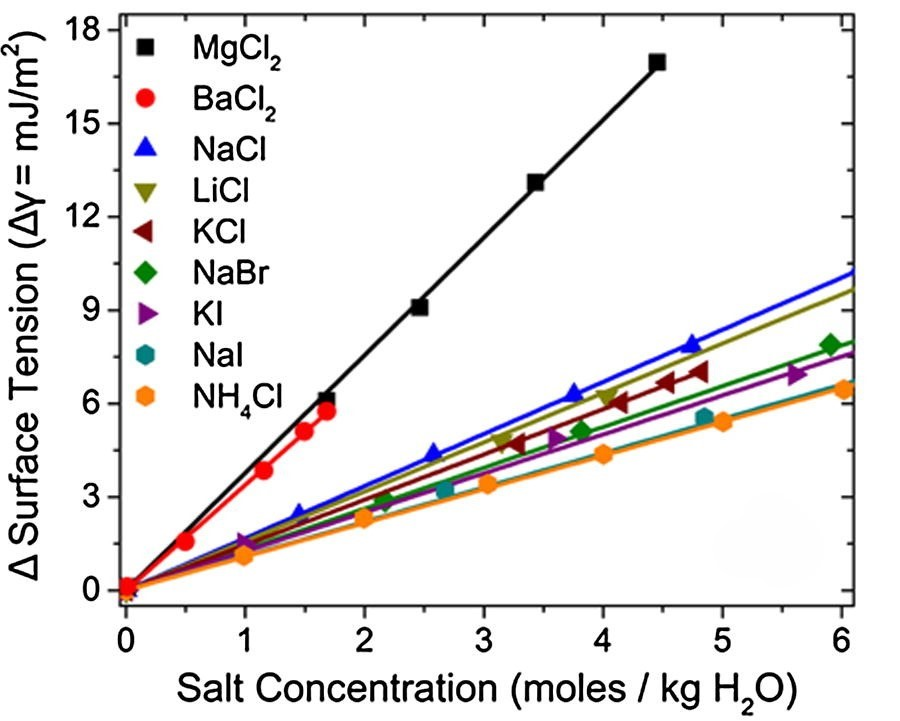
\includegraphics[width=0.7\linewidth]{images/ST_solute.jpg}
      \caption{Surface tension measurements of air/aqueous solution interfaces as a function of concentration for various salts. Image taken from \cite{okur2017jones}. }
      \label{fig:surf_tens_solute}
\end{figure}